\section{Speech Signal Processing}

\begin{frame}
\frametitle{Analog-to-Digital Conversion}
\begin{itemize}
\item Telephony since the 1950s limits the information bandwidth to 300-3400 Hz.
\item In normal conversational speech, the frequency content is mainly between 0-8000 Hz \cite{uysal2005bandwidth}.
\item We choose sampling rate $F_s$ = $2 \times 8000$ Hz = 16000 Hz.\\(Nyquist-Shannon sampling theorem)
\end{itemize}
\end{frame}

%----------------------------------------------------------------------------------------
%	Subsection
%----------------------------------------------------------------------------------------

\begin{frame}
\frametitle{Pre-emphasis}
\begin{itemize}
\item Pre-emphasis filter is essentially an \textbf{high-pass} filter.
\vspace{15pt}
\item Voiced speech naturally have an attenuation of $\sim$ 20 dB per decade due to physiological characteristics of the speech production system \cite{picone1993signal}.
\begin{itemize}
\item compensates this natural attenuation before spectral analysis.
\end{itemize}
\item Hearing is more sensitive to the components higher than 1 kHz.
\begin{itemize}
\item caters to human perception of sound
\end{itemize}
\end{itemize}
\end{frame}

%--------------------------------------------
%--------------------------------------------

\begin{frame}
A first-order FIR filter is widely implemented, including the previous group where $\alpha = 0.95$ \cite{EVW-report}.
\begin{equation}
y[n] = x[n] - \alpha x[n-1]
\end{equation}
\begin{itemize}
\item simple and efficient
\end{itemize}
\end{frame}

%--------------------------------------------
%--------------------------------------------

\begin{frame}
The \textcolor{orange_matlab}{orange dash-dot line} shows that frequencies below 500 Hz are severely suppressed even though frequencies above 3 kHz are successfully amplified.

\begin{figure}[H]
\centering
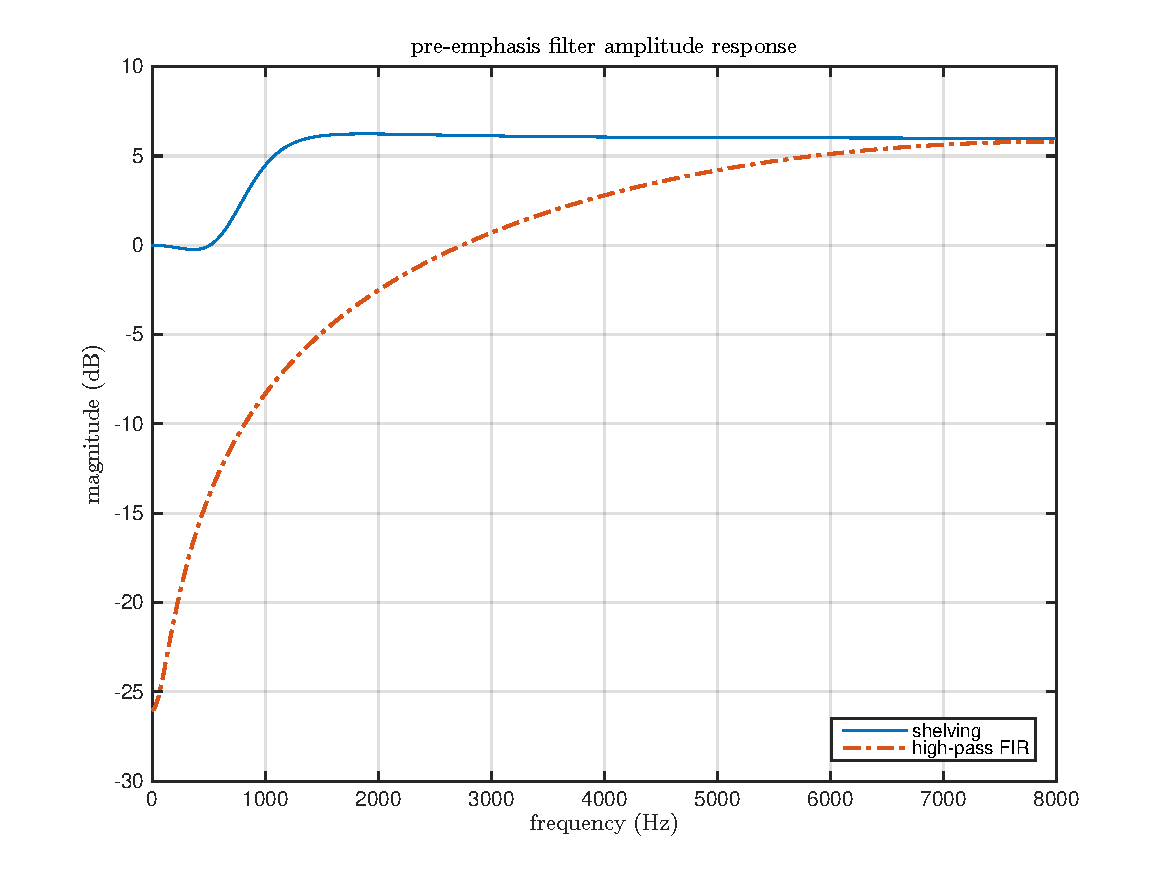
\includegraphics[width=3in, trim={0 0.6cm 0 0.6cm}, clip]{ang/pre_emphasis_filter}
\end{figure}
\end{frame}

%--------------------------------------------
%--------------------------------------------

\begin{frame}
Suggested by Professor Erik Weyer, we devised a second-order \textit{shelving filter} widely utilized in audio equalization to pre-emphasize the speech signal.

\begin{equation}
y[n] = \frac{1}{a_0} \Big( b_0 x[n] + b_1 x[n-1] + b_2 x[n-3] - a_1 y[n-1] - a_2 y[n-2] \Big)
\end{equation}
where
\begin{align}
&\begin{cases}
a_0 = 1\\
a_1 = -1.523796\\
a_2 = 0.649345
\end{cases}
&\begin{cases}
b_0 = 1.861856\\
b_1 = -3.102851\\
b_2 = 1.366544
\end{cases}
\end{align}
\end{frame}

%--------------------------------------------
%--------------------------------------------

\begin{frame}
Setting center frequency of transition band $F_c$ = 1000 Hz and gain $G$ = 6 dB, eventually we obtain an appropriate filter that effectively amplifies high-frequency components without attenuating low frequencies. The \textcolor{navy_matlab}{navy solid line} shows the frequency response of this shelving filter.

\begin{figure}[H]
\centering
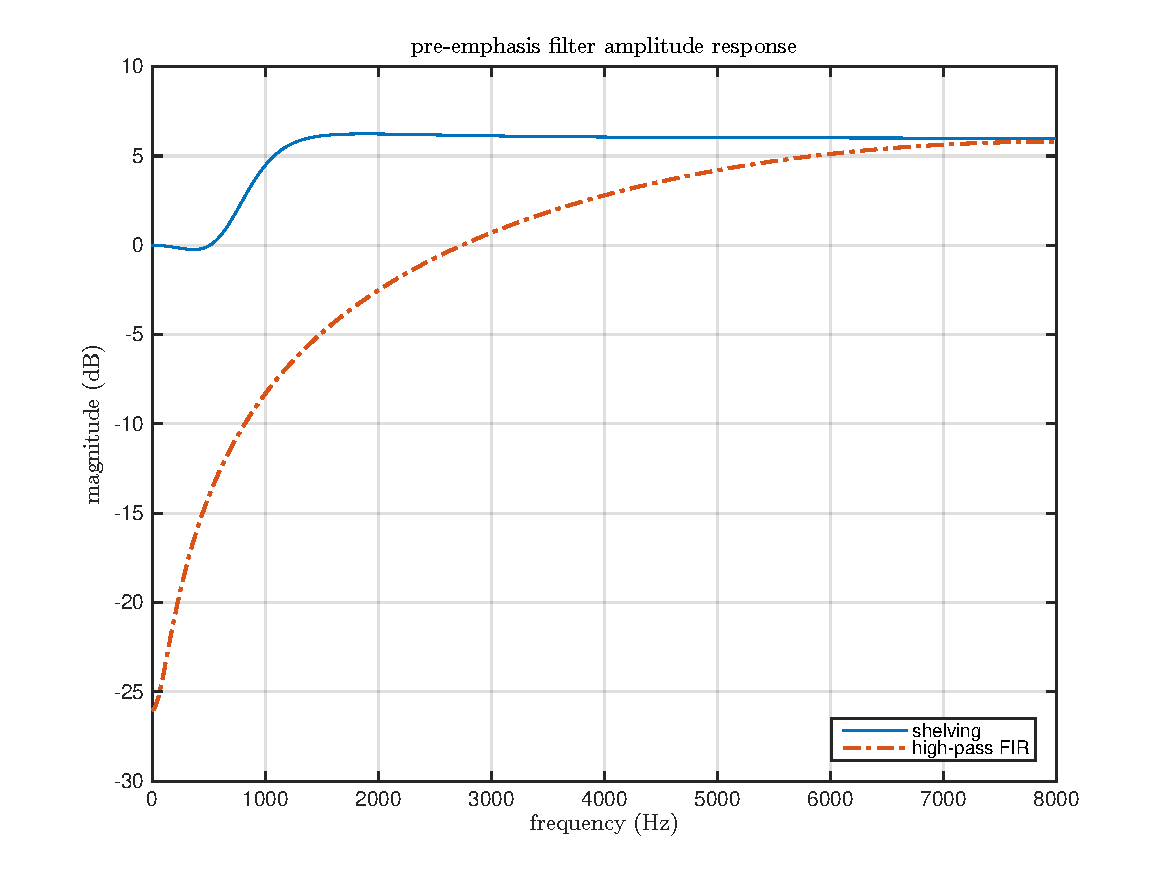
\includegraphics[width=3in, trim={0 0.6cm 0 0.6cm}, clip]{ang/pre_emphasis_filter}
\end{figure}
\end{frame}

%----------------------------------------------------------------------------------------
%	Subsection
%----------------------------------------------------------------------------------------

\begin{frame}
\frametitle{Framing \& Windowing}
Speech signals are time-varying signals, but due to the inertial motion of articulators (speech organs such as the tongue, lips and palate), speech can be considered statistically stationary in a short-time period ($\sim$ 30 ms) \cite{brandstein1995practical}.

\begin{align*}
30 \text{ ms} &\longrightarrow 480 \text{ samples per second}\\
&\longrightarrow N = 512 \text{ (Radix-2 FFT)}\\
\end{align*}
\end{frame}

%--------------------------------------------
%--------------------------------------------

\begin{frame}
The framing operation can be finished by multiplying the signal by a moving window.

\begin{equation}
s_j[n] =
\begin{cases}
w[n] s[n+jN] & n = 1, 2, \dots, N\\
0 & \text{otherwise}
\end{cases}
\end{equation}

The simplest and easiest-to-implement window is a rectangular window.
\begin{equation}
w[n] =
\begin{cases}
1, & n = 1, 2, \dots, N\\
0, & \text{otherwise}
\end{cases}
\end{equation}
\end{frame}

%--------------------------------------------
%--------------------------------------------

\begin{frame}
The selection of a proper window always involves a trade-off between \textbf{frequency resolution} and \textbf{spectral leakage}.

\begin{itemize}
\item the width of the mainlobe determines frequency resolution.
\item the gain of the sidelobes decides spectral leakage.
\end{itemize}
We chose an intermediate \textit{Hamming} window.

\begin{figure}[H]
\centering
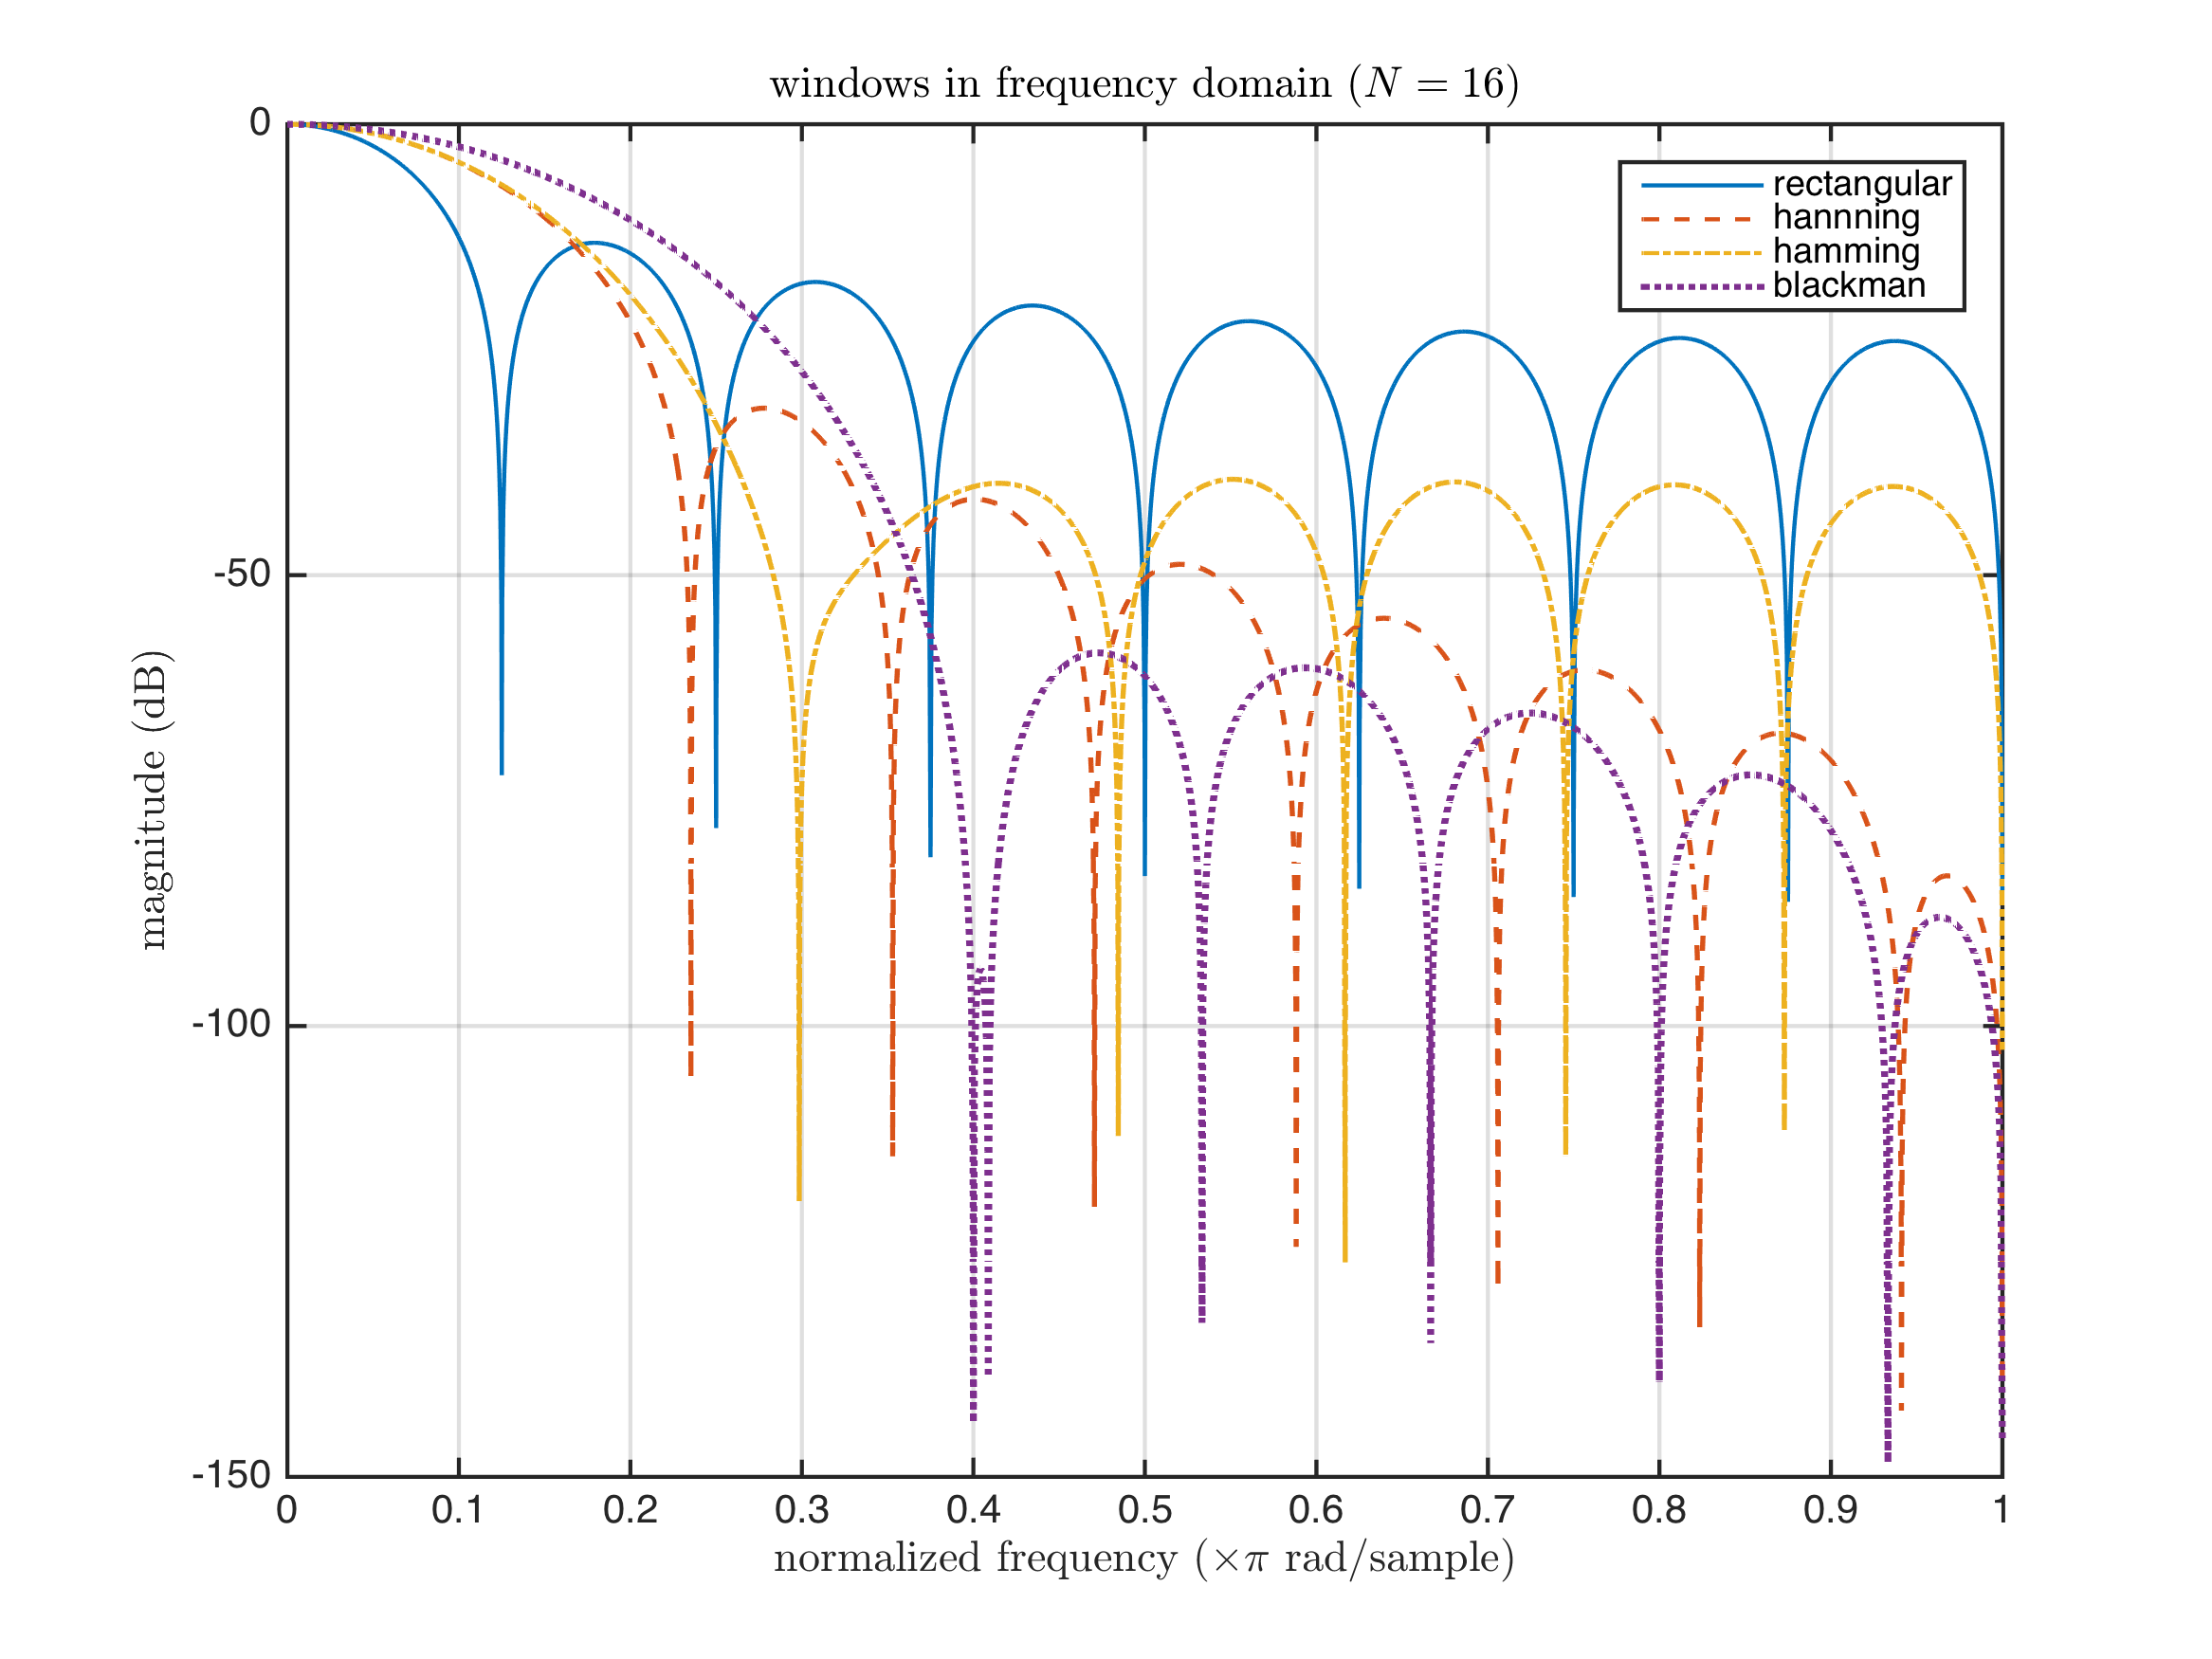
\includegraphics[width=3in, trim={0 0.6cm 0 0.6cm}, clip]{ang/windows_frequency}
\end{figure}
\end{frame}

%--------------------------------------------
%--------------------------------------------

\begin{frame}
Directly framing results in loss of information due to the bell shape of the Hamming window. Data points near two borders are severely attenuated (shown in \textcolor{red}{red dash-dot ellipse}).
\begin{figure}[H]
\centering
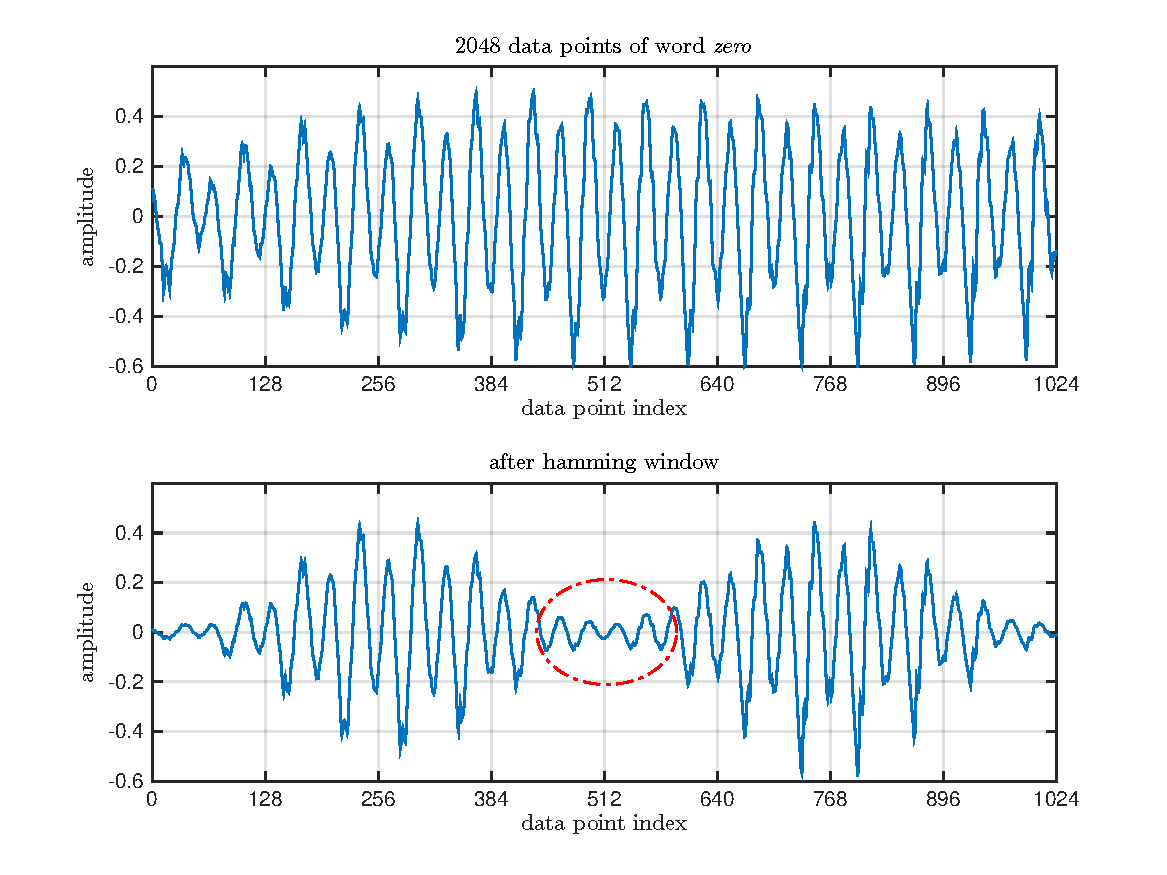
\includegraphics[width=3in, trim={0 0.6cm 0 0.6cm}, clip]{ang/hamming_bell_shape}
\end{figure}
\end{frame}

%--------------------------------------------
%--------------------------------------------

\begin{frame}
We overlapped each frame by half of the frame size primarily considering that data points most severely attenuated in current frame will have largest gain in the next frame. (shown in \textcolor{green_html}{green dash-dot rectangle})
\begin{figure}[H]
\centering
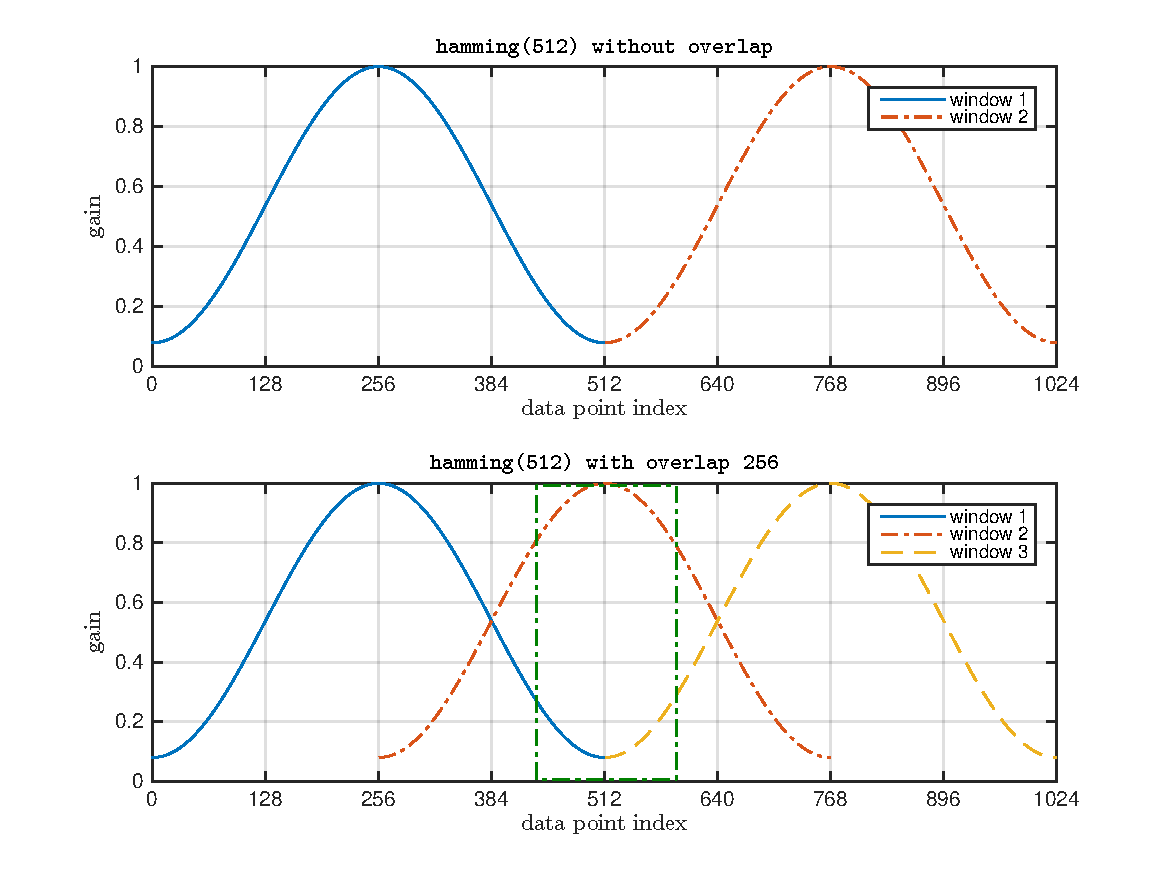
\includegraphics[width=3in, trim={0 0.6cm 0 0.6cm}, clip]{ang/hamming_overlap}
\end{figure}
\end{frame}

%----------------------------------------------------------------------------------------
%	Subsection
%----------------------------------------------------------------------------------------

\begin{frame}
\frametitle{Threshold}
\begin{itemize}
\item distinguish informative frames from silent frames
\item two metrics: frame \textit{energy} and frame \textit{zero-crossing count}
\end{itemize}

\begin{table}[H]
\centering
\caption{properties of different frame types}
\begin{tabu} to 0.9\textwidth {X[c]X[c]X[c]}
\toprule
Type &Energy &Zero-crossing count\\
\hline
Voiced &high &low\\
\hline
Unvoiced &low &high\\
\hline
Silent &low &low\\
\bottomrule
\end{tabu}
\end{table}
\end{frame}

%--------------------------------------------
%--------------------------------------------

\begin{frame}
\begin{figure}[H]
\centering
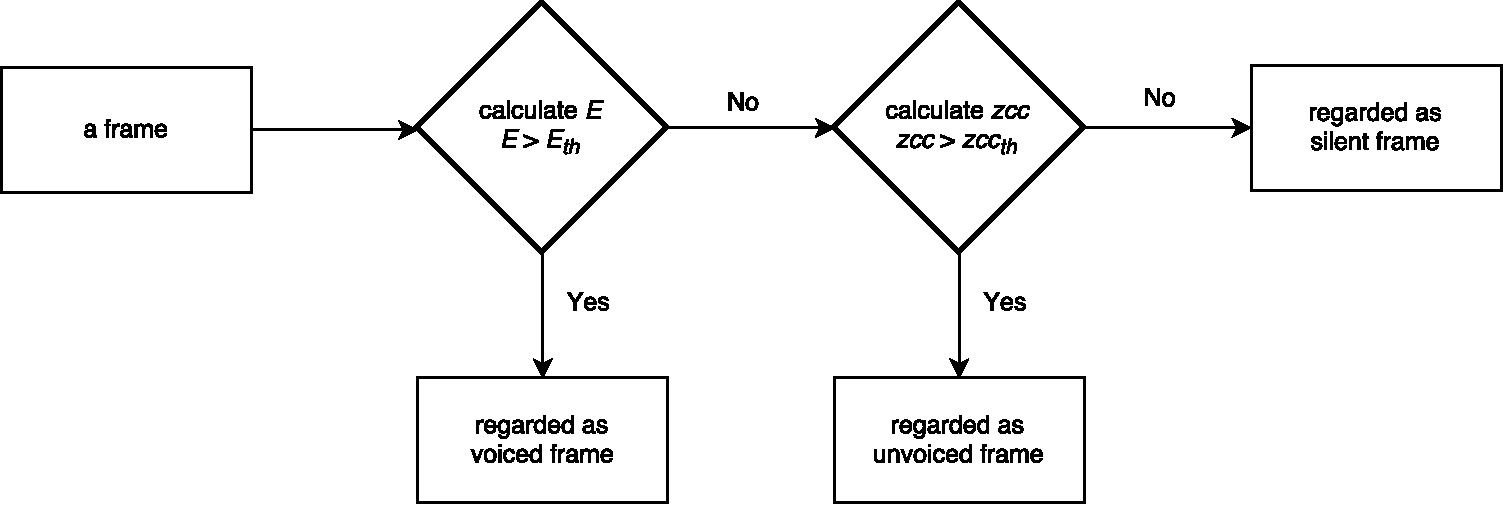
\includegraphics[width=\textwidth]{ang/threshold2}
\caption{decision-making strategy}
\end{figure}
\end{frame}

%----------------------------------------------------------------------------------------
%	Subsection
%----------------------------------------------------------------------------------------

\begin{frame}
\frametitle{Mel-frequency Cepstral Coefficients Extraction}
\begin{equation}
X[n] = \mathcal{F}^{-1} \left\{\log_{10} \left( |\mathcal{F}\{s[n]\}|^2 \right) \right\}
\end{equation}
\vspace{10pt}

The whole process to evaluate \textit{power cepstrum} can be divided into three procedures.
\begin{enumerate}
\item Compute the Discrete Fourier Transform $S_j[k]$ and corresponding power spectrum $\hat{S}_j[k]$ of a time-domain signal $s_j[n]$.
\item Take the logarithm of the power spectrum $\hat{S}_j[k]$.
\item Conduct inverse Fourier transform.
\end{enumerate}
\end{frame}

%--------------------------------------------
%--------------------------------------------

\begin{frame}
\begin{itemize}
	\item Human hearing responds to the entire critical band instead of individual frequencies in this band.
	\begin{itemize}
		\item MFCC calculates the total power within each certain mel-scale band prior to log scaling.
	\end{itemize}
	\item MFCC substitutes Discrete Cosine Transform for inverse Fourier transform to reduce the computational complexity.
\end{itemize}
\vspace{10pt}

MFCC extraction process
\begin{enumerate}
\item Power spectrum
\item Bank filtering
\item Log scaling
\item Discrete cosine transform
\end{enumerate}
\end{frame}

%--------------------------------------------
%--------------------------------------------

\begin{frame}
\frametitle{I. Power spectrum}

Discrete Fourier Transform constitutes the cornerstone of spectrum analysis.
\begin{equation}
S_j[k] = \sum_{n=1}^{N} s_j[n] W_N^{(n-1) k} \quad k = 1, 2, \dots, N
\end{equation}
\begin{equation}
W_N = e^{\frac{- 2\pi i}{N}}
\end{equation}

\begin{itemize}
	\item The computations required by DFT increase dramatically as length $N$ increases.
	\begin{itemize}
		\item Infeasible to directly implement on large sequences.
	\end{itemize}
	\item Fast Fourier Transform makes implementation of DFT practical in real-time processing.
	\begin{itemize}
		\item Radix-2 algorithm restricts the length of input sequence to $2^n$.
	\end{itemize}
\end{itemize}
\end{frame}

%--------------------------------------------

\begin{frame}
The DFT $X[k]$ of a real sequence $x[n] \in \mathbb{R}$ is a conjugate symmetric sequence (from ELEN90058 \textit{Signal Processing} Workshop 3).
\begin{equation}
X[k] = X^*[\langle-k\rangle_{N}] = X^*[N-k]
\end{equation}

Last $(\frac{N}{2} - 1)$ points can be discarded when computing the power spectrum.
\begin{equation}
\hat{S}_j[k] = |S_j(k)|^2 \quad k = 1, 2, \dots, \frac{N}{2} + 1
\end{equation}
\end{frame}

%--------------------------------------------
%--------------------------------------------

\begin{frame}
\frametitle{II. Bank Filtering}
Total power within each mel-scale bank
\begin{equation}
X_j[m] = \sum^{\frac{N}{2} + 1}_{k=1} \hat{S}_j[k] H_{mel}[m, k] \quad m = 1, 2, \dots, M
\end{equation}
where $H_{mel}[m, k]$ is the gain of the $k$-th power spectrum data point within bank $m$.
\end{frame}

%--------------------------------------------

\begin{frame}
\begin{equation}
H_{mel}[m, k] =
\begin{cases}
0 &f_{d2c}(k) \le f[m-1]\\
\displaystyle\frac{k - f[m-1]}{f[m] - f[m-1]} &f[m-1] < f_{d2c}(k) \le f[m]\\
\displaystyle\frac{f[m+1] - k}{f[m+1] - f[m]} &f[m] < f_{d2c}(k) \le f[m+1]\\
0 &f_{d2c}(k) > f[m+1]
\end{cases}
\end{equation}
where $f_{d2c}(k) = (k-1) \cdot \frac{F_s}{N}$ transforming the index $k$ of DFT into continuous-time frequency.\\
\vspace{10pt}
Frequency boundaries $f[m]$ ($m = 0, 1, \dots, M+1$) are equally spaced in mel-scale. We take $f[0]$ = 0 Hz and $f[M+1] = \frac{F_s}{2}$ = 8000 Hz as per the system specification and popular number of banks $M = 20$ \cite{davis1980comparison}.
\end{frame}

%--------------------------------------------

\begin{frame}
\begin{figure}[H]
\centering
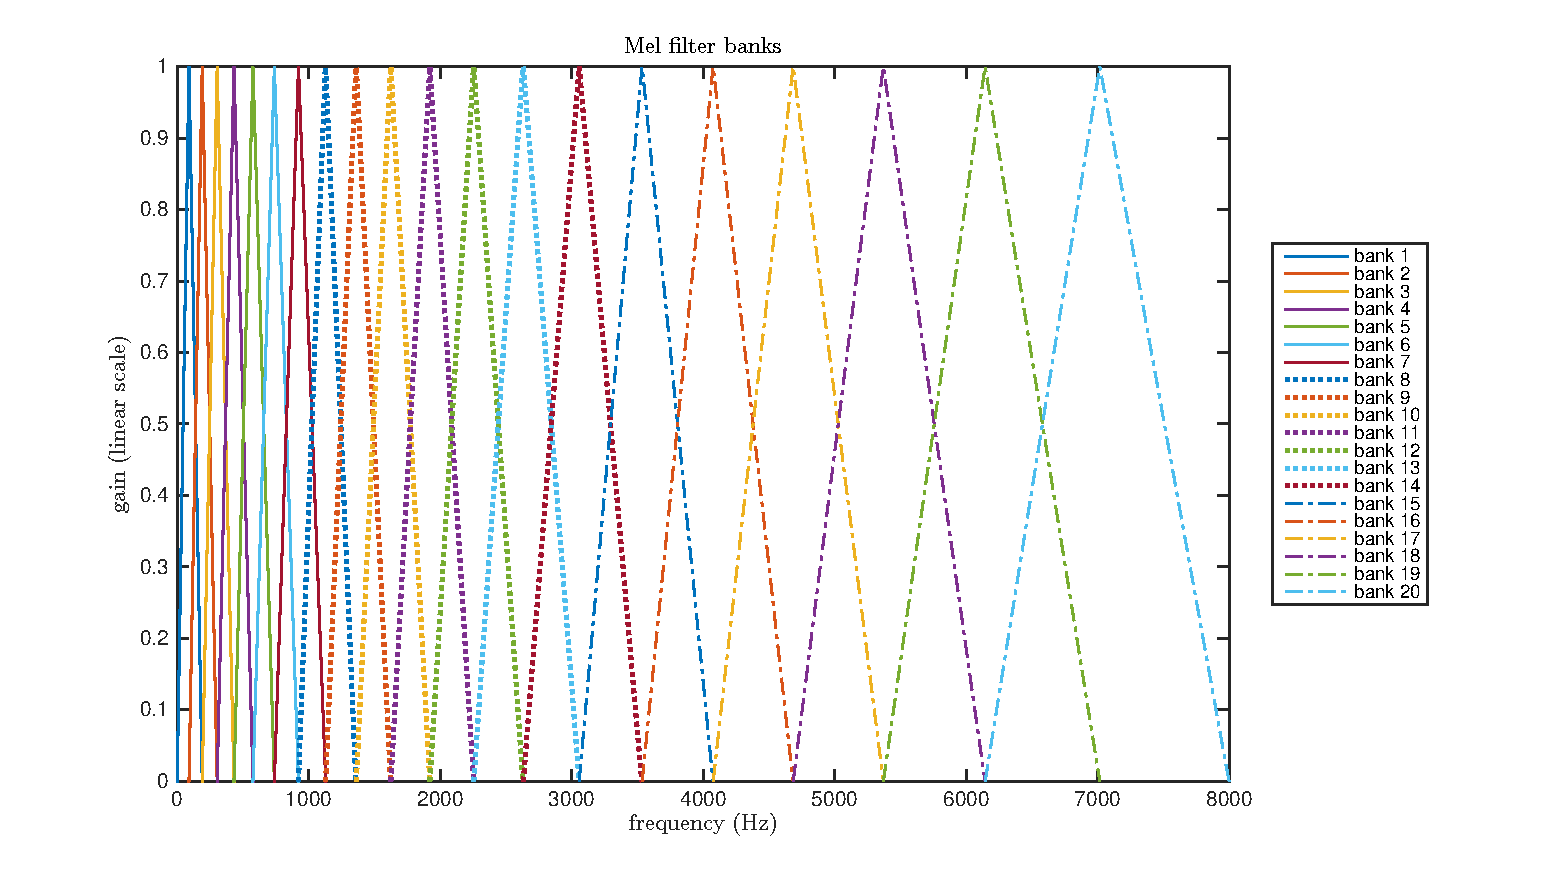
\includegraphics[width=0.9\textwidth, trim={0 0.6cm 0 0.6cm}, clip]{ang/mel_triangle}
\end{figure}

$H_{mel}$ is essentially a band-pass filter for each bank $m$. $H_{mel}$ offers maximal gain 1 at the `central frequency' of bank $m$ and then linearly decreases to 0 until reaching adjacent critical frequencies (the `central frequency' of bank $m-1$ and bank $m+1$).
\end{frame}

%--------------------------------------------

\begin{frame}
\begin{enumerate}
\item Each power spectrum data point $\hat{S}_j[k]$ (\textcolor{gold_matlab}{gold circle $\circ$}) is multiplied by the corresponding gain $H_{mel}[m, k]|_{m=9}$ (\textcolor{orange_matlab}{orange asterisk $*$}).
\item \textcolor{orange_matlab}{Orange crosses $\times$} represent the filtered power spectrum.
\item Total power within bank $m=9$ is the sum of all filtered power data points.
\end{enumerate}

\begin{figure}[H]
\centering
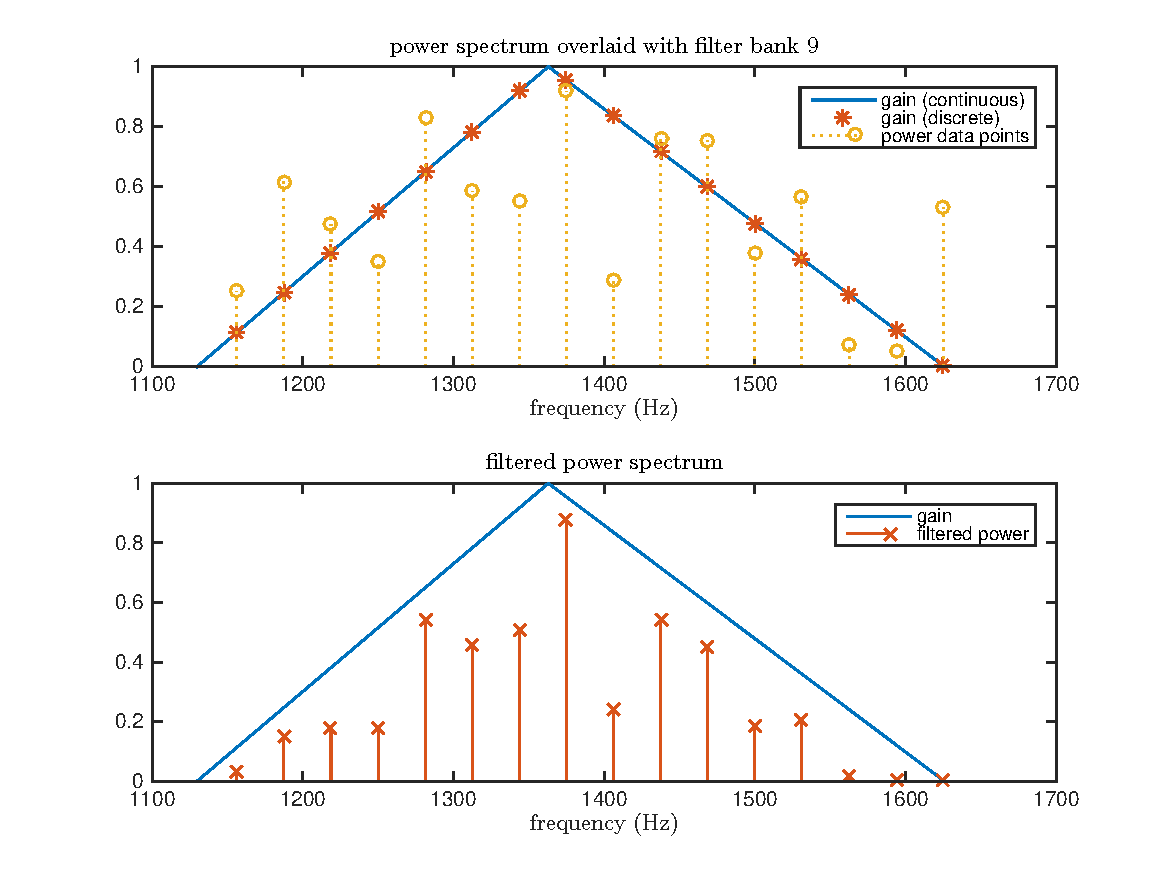
\includegraphics[width=3in, trim={0 0.6cm 0 0.6cm}, clip]{ang/bank_filter_demostration}
\end{figure}
\end{frame}

%--------------------------------------------
%--------------------------------------------

\begin{frame}
\frametitle{III. Log Scaling}
\begin{equation}
\hat{X}_j[m] = \log_{10}(X_j[m]) \quad m = 1, 2, \dots, M
\end{equation}

\begin{enumerate}
\item Log scaling makes the system more resilient to both very quiet and very loud sound.
\item Log scale in dB imitates human nonlinear perception to loudness \cite{farin2008mathematical}.
\item Without taking logarithm, recognition accuracy is severely reduced \cite{tan2008automatic}.
\end{enumerate}
\end{frame}

%--------------------------------------------
%--------------------------------------------

\begin{frame}
\frametitle{IV. Discrete Cosine Transform}
IDFT is replaced by discrete cosine transform (DCT) due to the symmetric and real characteristic of log power spectrum $\hat{X}_j[m]$ \cite{picone1993signal, iser2008bandwidth}.
\begin{equation}
\hat{C}_j[n] = \sqrt{\frac{2}{M}} \sum^{M}_{m=1} \hat{X}_j[m] \cos \left( \frac{\pi}{M} (m - 0.5) (n-1) \right) \quad n = 1, 2, \dots, F
\end{equation}

\begin{itemize}
	\item The order of DCT ($F$) determines the amount of MFCCs. \cite{tan2008automatic}
	\begin{itemize}
		\item Higher-order coefficients incorporates excitation information.
		\item Lower-order coefficients indicate the slowly varying vocal tract. (more useful for speech recognition)
	\end{itemize}
	\item European Telecommunications Standards Institute adopts $F = 13$ in their speech recognition standard \cite{etsi2001202}.
	\item We also condense the $M$-point sequence $\hat{X}_j[m]$ into a shorter $F$-point sequence $\hat{C}_j[n]$. The choice of $F$ will be further discussed in \textit{Design \& Performance} section.
\end{itemize}
\end{frame}
